\documentclass[11pt,a4paper]{ctexart}
\usepackage{geometry}
\geometry{left=2cm,right=2cm,top=2.5cm,bottom=2.5cm}
\usepackage{amsmath}
\usepackage{amssymb}
\usepackage{amsfonts}
\usepackage{bm}
\usepackage{tikz}
\usetikzlibrary{decorations.pathmorphing}

\begin{document}

% 试卷页眉与标题
\begin{center}
    {\LARGE\bfseries 中国科学技术大学} \\[0.6em]
    {\Large\bfseries 2025--2026学年第一学期期末考试试卷（A卷）}
\end{center}

\vspace{1em}

% 学生信息登记表
\noindent
\textbf{考试科目：} 现代控制理论 \hfill \textbf{考试时间：} 2026.1.13 \hfill \textbf{得分：} \underline{\hspace{2cm}} \\
\textbf{学生所在系：} \underline{\hspace{3.5cm}} \hfill \textbf{姓名：} \underline{\hspace{3.5cm}} \hfill \textbf{学号：} \underline{\hspace{4.5cm}}

\vspace{1.5em}

% 得分统计表
\noindent
\begin{table}[h]
\centering
\small
\def\arraystretch{1.5}
\begin{tabular}{|c|p{1.2cm}|p{1.2cm}|p{1.2cm}|p{1.2cm}|p{1.2cm}|p{1.2cm}|p{1.5cm}|}
\hline
\textbf{题号} & \hfil \textbf{一} & \hfil \textbf{二} & \hfil \textbf{三} & \hfil \textbf{四} & \hfil \textbf{五} & \hfil \textbf{六} & \hfil \textbf{总分} \\ \hline
\textbf{得分} & & & & & & & \\ \hline
\end{tabular}
\end{table}

\vspace{1.5em}

% 试题部分
\noindent
\textbf{一、（15分）} 如图所示弹簧-质量系统。三个弹簧、两个滑块相间串接，两端固定在墙壁上。计各滑块的质量分别为 $m_1$、$m_2$，弹簧的弹性系数分别为 $k_1$、$k_2$、$k_3$，忽略滑块与地面的摩擦。以作用在滑块上的力 $u_1$、$u_2$ 为输入，滑块的位移 $y_1$、$y_2$ 为输出，试选择合适的状态变量，建立系统的状态空间方程。

\vspace{1em}
\begin{center}
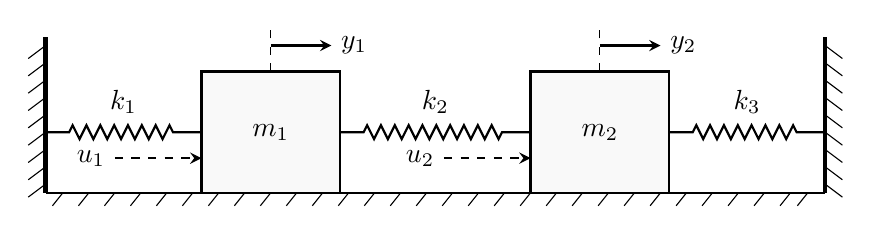
\begin{tikzpicture}[scale=1.1]
    % 左侧墙壁
    \draw[ultra thick] (0,-0.6) -- (0,1.2);
    \foreach \y in {-0.5,-0.3,-0.1,0.1,0.3,0.5,0.7,0.9,1.1}
        \draw (0,\y) -- (-0.2,\y-0.15);
        
    % 右侧墙壁
    \draw[ultra thick] (9,-0.6) -- (9,1.2);
    \foreach \y in {-0.5,-0.3,-0.1,0.1,0.3,0.5,0.7,0.9,1.1}
        \draw (9,\y) -- (9.2,\y-0.15);
        
    % 地面
    \draw[thick] (0,-0.6) -- (9,-0.6);
    \foreach \x in {0.2,0.5,0.8,1.1,1.4,1.7,2.0,2.3,2.6,2.9,3.2,3.5,3.8,4.1,4.4,4.7,5.0,5.3,5.6,5.9,6.2,6.5,6.8,7.1,7.4,7.7,8.0,8.3,8.6,8.8}
        \draw (\x,-0.6) -- (\x-0.12,-0.75);

    % 滑块 m1
    \draw[thick, fill=gray!5] (1.8,-0.6) rectangle (3.4,0.8);
    \node at (2.6,0.1) {$m_1$};
    
    % 滑块 m2
    \draw[thick, fill=gray!5] (5.6,-0.6) rectangle (7.2,0.8);
    \node at (6.4,0.1) {$m_2$};

    % 弹簧 k1
    \draw[thick, decoration={zigzag, pre length=3mm, post length=3mm, segment length=5}, decorate] (0,0.1) -- (1.8,0.1);
    \node[above] at (0.9,0.2) {$k_1$};
    
    % 弹簧 k2
    \draw[thick, decoration={zigzag, pre length=3mm, post length=3mm, segment length=5}, decorate] (3.4,0.1) -- (5.6,0.1);
    \node[above] at (4.5,0.2) {$k_2$};
    
    % 弹簧 k3
    \draw[thick, decoration={zigzag, pre length=3mm, post length=3mm, segment length=5}, decorate] (7.2,0.1) -- (9,0.1);
    \node[above] at (8.1,0.2) {$k_3$};

    % 输入外力 u1, u2
    \draw[->, >=stealth, thick, dashed] (0.8,-0.2) -- (1.8,-0.2);
    \node[left] at (0.8,-0.2) {$u_1$};
    \draw[->, >=stealth, thick, dashed] (4.6,-0.2) -- (5.6,-0.2);
    \node[left] at (4.6,-0.2) {$u_2$};

    % 位移指示 y1
    \draw[dashed] (2.6,0.8) -- (2.6,1.3);
    \draw[->, >=stealth, thick] (2.6,1.1) -- (3.3,1.1);
    \node[right] at (3.3,1.1) {$y_1$};

    % 位移指示 y2
    \draw[dashed] (6.4,0.8) -- (6.4,1.3);
    \draw[->, >=stealth, thick] (6.4,1.1) -- (7.1,1.1);
    \node[right] at (7.1,1.1) {$y_2$};
\end{tikzpicture}
\end{center}

\vspace{1.5em}

\noindent
\textbf{二、（15分）} 已知单输入--单输出系统：
\begin{equation*}
    \dot{\bm{x}}(t) = \begin{bmatrix} 0 & 1 & 0 \\ 0 & 0 & 1 \\ 0 & -4 & -4 \end{bmatrix} \bm{x}(t) + \begin{bmatrix} 0 \\ 0 \\ 1 \end{bmatrix} u(t)
\end{equation*}
\begin{equation*}
    y(t) = \begin{bmatrix} a & -1 & 1 \end{bmatrix} \bm{x}(t) + u(t)
\end{equation*}
1. 分析参数 $a$ 对系统稳定性（渐近稳定，李雅普诺夫意义下的稳定、BIBO 稳定）的影响；\\
2. 分析参数 $a$ 对系统的能控性和能观性的影响。

\vspace{1.5em}

\noindent
\textbf{三、（12分）} 陈述定常系统末端时刻固定、末端状态受等式约束、控制向量 $\bm{u}(t)$ 受不等式约束时，极小值原理的问题提法和基本结论（最优控制 $\bm{u}^*(t)$、最优轨迹 $\bm{x}^*(t)$，使性能泛函达到极值 $J^*$，包括求解所需的方程和条件）。

\newpage % 适配第二页排版

\noindent
\textbf{四、（22分）} 系统是传递函数为
\begin{equation*}
    \hat{g}(s) = \frac{s + 3}{s^2 + 3s + 2}
\end{equation*}
的单输入单输出二维系统，在分别选取状态反馈
\begin{equation*}
    u_1 = r - \begin{bmatrix} -3 & 2 \end{bmatrix} \bm{x}, \quad u_2 = r - \begin{bmatrix} 1 & 1 \end{bmatrix} \bm{x}
\end{equation*}
的情况下，系统的单位阶跃响应分别为
\begin{equation*}
    y_1(t) = 1 - e^{-t}, \quad t \ge 0 \quad \text{及} \quad y_2(t) = 0.5 - 0.5e^{-0.5t}, \quad t \ge 0
\end{equation*}
求原系统的状态空间方程。

\vspace{1.5em}

\noindent
\textbf{五、（22分）} 已知系统的状态方程：
\begin{align*}
    \dot{x}_1 &= x_2, \quad x_1(0) = 1 \\
    \dot{x}_2 &= u, \quad x_2(0) = -1
\end{align*}
试求使性能指标
\begin{equation*}
    J = \int_0^\infty (x_1^2 + 2x_1x_2 + 2x_2^2 + u^2) \, dt
\end{equation*}
最小的最优控制 $u^*(t)$、最优轨迹 $\bm{x}^*(t)$ 及最优性能指标 $J^*$。

\vspace{1.5em}

\noindent
\textbf{六、（14分）} 对线性定常系统 $\{\bm{A}, \bm{b}, \bm{c}\}$ 证明以下结论：\\
1. 状态变换不改变系统的传递函数；\\
2. 用渐近状态观测器得到的状态估值，替代真实状态进行状态反馈，不影响状态反馈的效果（即从指令输入 $r$ 至系统输出 $y$ 的传递函数完全一致）。

\end{document}
